\documentclass[tikz]{standalone}
\usepackage{pgfplots}
\pgfplotsset{compat=1.15}
\usepackage{mathrsfs}
\usetikzlibrary{arrows,calc}
\usepackage{tkz-euclide}
\pagestyle{empty}

\definecolor{AngleClr}{rgb}{0,0.39215686274509803,0}
\definecolor{ShapeClr}{rgb}{0.6,0.2,0}
\definecolor{SquareClr}{RGB}{250, 248, 217}
\definecolor{GreenDist}{RGB}{7,122,7}

\begin{document}

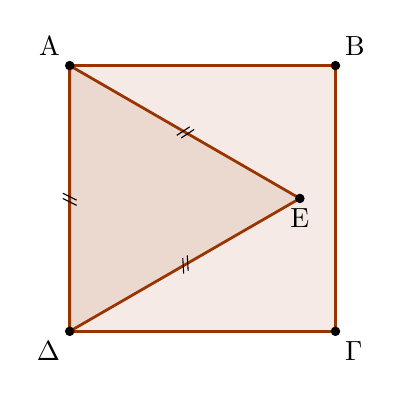
\begin{tikzpicture}[scale=.75]
\tkzSetUpLine[line width=1pt,color=black]
\tkzSetUpPoint[fill=black]

\tkzDefPoints{0/0/D,4.5/0/C,4.5/4.5/B,0/4.5/A}

\tkzDefTriangle[equilateral](A,D) \tkzGetPoint{E}


\tkzFillPolygon[fill=ShapeClr,fill opacity=0.1](A,B,C,D)
\tkzFillPolygon[fill=ShapeClr,fill opacity=0.1](A,D,E)

\tkzDrawPolygon[color=ShapeClr](A,B,C,D)
\tkzDrawPolygon[color=ShapeClr](A,D,E)

\tkzDrawPoints[size=3](A,B,C,D,E)

\tkzLabelPoint[above left](A){$\rm A$}
\tkzLabelPoint[above right](B){$\rm B$}
\tkzLabelPoint[below right](C){$\rm \Gamma$}
\tkzLabelPoint[below left](D){$\rm \Delta$}
\tkzLabelPoint[below](E){$\rm E$}


\tkzMarkSegments[mark=s||,size=2.5](A,D D,E A,E)

\end{tikzpicture}

\end{document}
